\documentclass[11pt,twoside,a4paper]{article}
\usepackage{ctex}
\usepackage[utf8]{inputenc}
\usepackage{amsmath}
\title{从零开始写vio}
\author{kohill}
\date{October 2019}

\usepackage{natbib}
\usepackage{graphicx}

\begin{document}
\section{VIO文献阅读}
\begin{figure}[htbp]
    \centering
    
\includegraphics[width=0.9\linewidth]{001.png}
    % \caption{}    
\end{figure}

>. 视觉与IMU融合的优势
\begin{itemize}
    \item IMU短期精度高,但是长时间误差大,总体来说视觉长时间更加稳定. 
    \item 在纯旋转的时候,视觉跟踪容易丢失,但是IMU对纯旋转不敏感。
\end{itemize}

>. 有哪些常见的视觉+IMU方案

基于滤波的方法,例如MSCKF, 基于优化的方法,例如VINS,OKVIS, VI-ORB等。基于深度学习的比如VINet(Visual-inertial odometry as a sequence-to-sequence learning problem);
DeepVO:(A Deep Learning approach for Monocular Visual Odometry)等。

VINS在VR领域有着比较成熟的应用,例如谷歌的ARCore。


\section{四元数和李代数更新}
运行结果如图\ref{fig:executeresult}所示,代码见main.cpp
\begin{figure}[h]
    \centering
    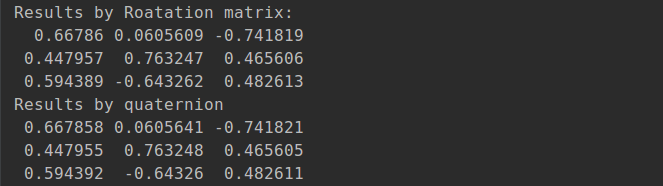
\includegraphics[width=0.9\linewidth]{003.png}
    \caption{运行结果}    
    \label{fig:executeresult}
\end{figure}



\section{其他导数}
\begin{figure}[h!]
    \centering
    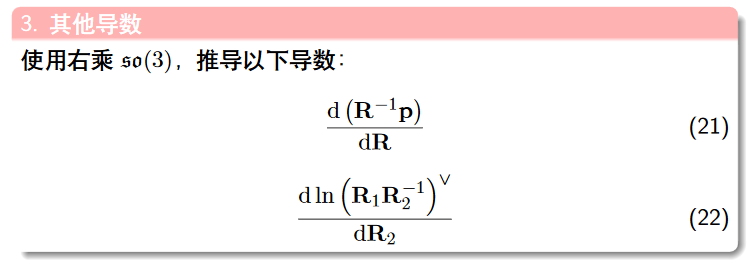
\includegraphics[width=0.9\linewidth]{004.png}
    % \caption{}    
\end{figure}
\begin{align}
    \frac{d(\textbf{R}^{-1}p)}{d\textbf{R}}
    &=\lim_{\phi \to 0}{\frac{(\textbf{R} \exp(\phi^{\wedge}) )^{-1}p - \textbf{R}^{-1}p}{\phi}} \\
    &=\lim_{\phi \to 0}{\frac{ \exp((-\phi)^{\wedge}) \textbf{R}^{-1}  p - \textbf{R}^{-1}p}{\phi}} \\
    &\approx \lim_{\phi \to 0}{\frac{ (\textbf{I} + (-\phi)^{\wedge}) \textbf{R}^{-1}  p - \textbf{R}^{-1}p}{\phi}} \\
    &= \lim_{\phi \to 0}{\frac{ (-\phi)^{\wedge} \textbf{R}^{-1}  p}{\phi}} \\
    &= \lim_{\phi \to 0}{\frac{ (\mathbf{R}^{-1}p)^{\wedge}\phi}{\phi}}\\
    &= (\mathbf{R}^{-1}p)^{\wedge}
\end{align}

\begin{align}
    \frac{\ln(\mathbf{R}_1\mathbf{R}_2^{-1})^\vee}{d\mathbf{R}_2} 
    &= \lim_{\phi \to 0} 
    \frac{\ln(\mathbf{R}_1(\mathbf{R}_2\exp(\phi^\wedge))^{-1})^\vee - \ln(\mathbf{R}_1\mathbf{R}_2^{-1})^\vee}{\phi} \\
    &= \lim_{\phi \to 0} 
    \frac{\ln(\mathbf{R}_1\exp((-\phi)^\wedge)\mathbf{R}_2^{-1})^\vee - \ln(\mathbf{R}_1\mathbf{R}_2^{-1})^\vee}{\phi} \\
    &= \lim_{\phi \to 0} 
    \frac{\ln(\mathbf{R}_1\mathbf{R}_2^{-1}\mathbf{R}_2\exp((-\phi)^\wedge)\mathbf{R}_2^{-1})^\vee - \ln(\mathbf{R}_1\mathbf{R}_2^{-1})^\vee}{\phi} \\
    &= \lim_{\phi \to 0}
    \frac{\ln(\mathbf{R}_1\mathbf{R}_2^{-1}\exp((\mathbf{R_2}\phi)^\wedge))^\vee - \ln(\mathbf{R}_1\mathbf{R}_2^{-1})^\vee}{\phi} \\
    &= \lim_{\phi \to 0}
    \frac{\ln(\mathbf{R}_1\mathbf{R}_2^{-1})^\vee + \mathbf{J}_r^{-1} \mathbf{R_2}\phi - \ln(\mathbf{R}_1\mathbf{R}_2^{-1})^\vee}{\phi} \\
    &= \mathbf{J}_r^{-1}(\ln{(\mathbf{R}_1\mathbf{R}_2^{-1})^\vee}) \mathbf{R}_2
\end{align}
\end{document}